\documentclass[a4paper,footsepline]{scrartcl}

\usepackage[utf8]{inputenc}
\usepackage[T1]{fontenc}
\usepackage{lmodern}

%##### English
\usepackage[english]{fancyref}
\usepackage[USenglish]{babel}

%#### Deutsch
%\usepackage[ngerman]{babel}
%\usepackage[german]{fancyref}

%#### Usepackage #####

\usepackage{uepage} 
\usepackage{amssymb}

\usepackage{courier}
\usepackage{hyperref}
\usepackage{listings}
\usepackage{color}
\usepackage{tikz}
\usepackage{wasysym}
\usepackage{framed}
\usetikzlibrary{arrows, automata}
\usepackage{ marvosym }
\usepackage{placeins}


\newcommand{\reals}{\mathbb{R}}
\newcommand{\vect}[1]{\begin{pmatrix} #1\end{pmatrix}}

\areaset{15cm}{28cm}

%#### Title page #####
\title{Cyber Physical Systems: Stochastic foundations LU}
\subject{Term Project - Design Document}

\author{
	\authorname{Mathias Lechner, Benjamin Binder} \\
	\authorname{Johannes Obermüller, Lukas Hartung} \\
	\studentnumber{1225134, 1226121, 1126799} \\
	\curriculum{066 938}\\
	\email{e1225134@student.tuwien.ac.at, e1226121@student.tuwien.ac.at}\\
	\email{e1126799@student.tuwien.ac.at}\\\\
}
\date{\today}


%### Start of Document
\begin{document}


\maketitle
\section*{Problem statement and requirements}
The task of this project is to implement the \textbf{control\_system} of the provided quadcopter simulation. The \textbf{control\_system} get measurement values from the quadcopter model as input and should provide PWM commands for the motors of the quadcopter as output, such that the quadcopter:
\begin{enumerate}
	\item does not crash on the ground or with an obstacle
	\item pass through all the waypoints
	\item finally reaches the target position
\end{enumerate}
The side condition is that condition 2) and 3) should be achieved as fast as possible. At the start of the simulation the quadcopter is placed to a fixed starting position.
\vspace{0.2cm}\\
The measurement inputs of the \textbf{control\_system} include data from:
\begin{itemize}
	\item a 3-axis gyroscope
	\item a 3-axis accelerometer
	\item latitude, longitude and altitude values from a GPS sensor
	\item a sonar based distance sensor that points to the bottom of the quadcopter
\end{itemize}
The GPS sensor provide new data ever 200 ms, the sonar sensor every 100ms. The update frequency of the gyroscope and accelerometer is a lot higher (maybe add exact value here).
\vspace{0.2cm}\\
A PI-controller is provided that takes absolute pitch, roll and yaw-differences values and controls the pose of the quadcopter accordingly by generating the PWM signals for the motors. \\
To accomplish this, the PI-controller needs the current pose of the quadcopter, thus this pose is an additional measurement that is provided to the \textbf{control\_system}. \\
So the task of this project includes building a \emph{state estimator} for the pose of the quadcopter based on the given measurement, i.e. this additional measurement of the pose needs to be replaced by a estimated pose based on the given measurements.
\FloatBarrier
\section*{Design: components}
The components of our solution will be designed according to figure (\ref{fig:layers}). 
\begin{figure}
	\centering
	\includegraphics[width=0.8\textwidth]{images/figure.png}
	\caption{Three-level architecture of a goal-based agent (taken from the assignment document)}
	\label{fig:layers}
\end{figure}
\begin{figure}
	\centering
	\resizebox{\textwidth}{!}{%
	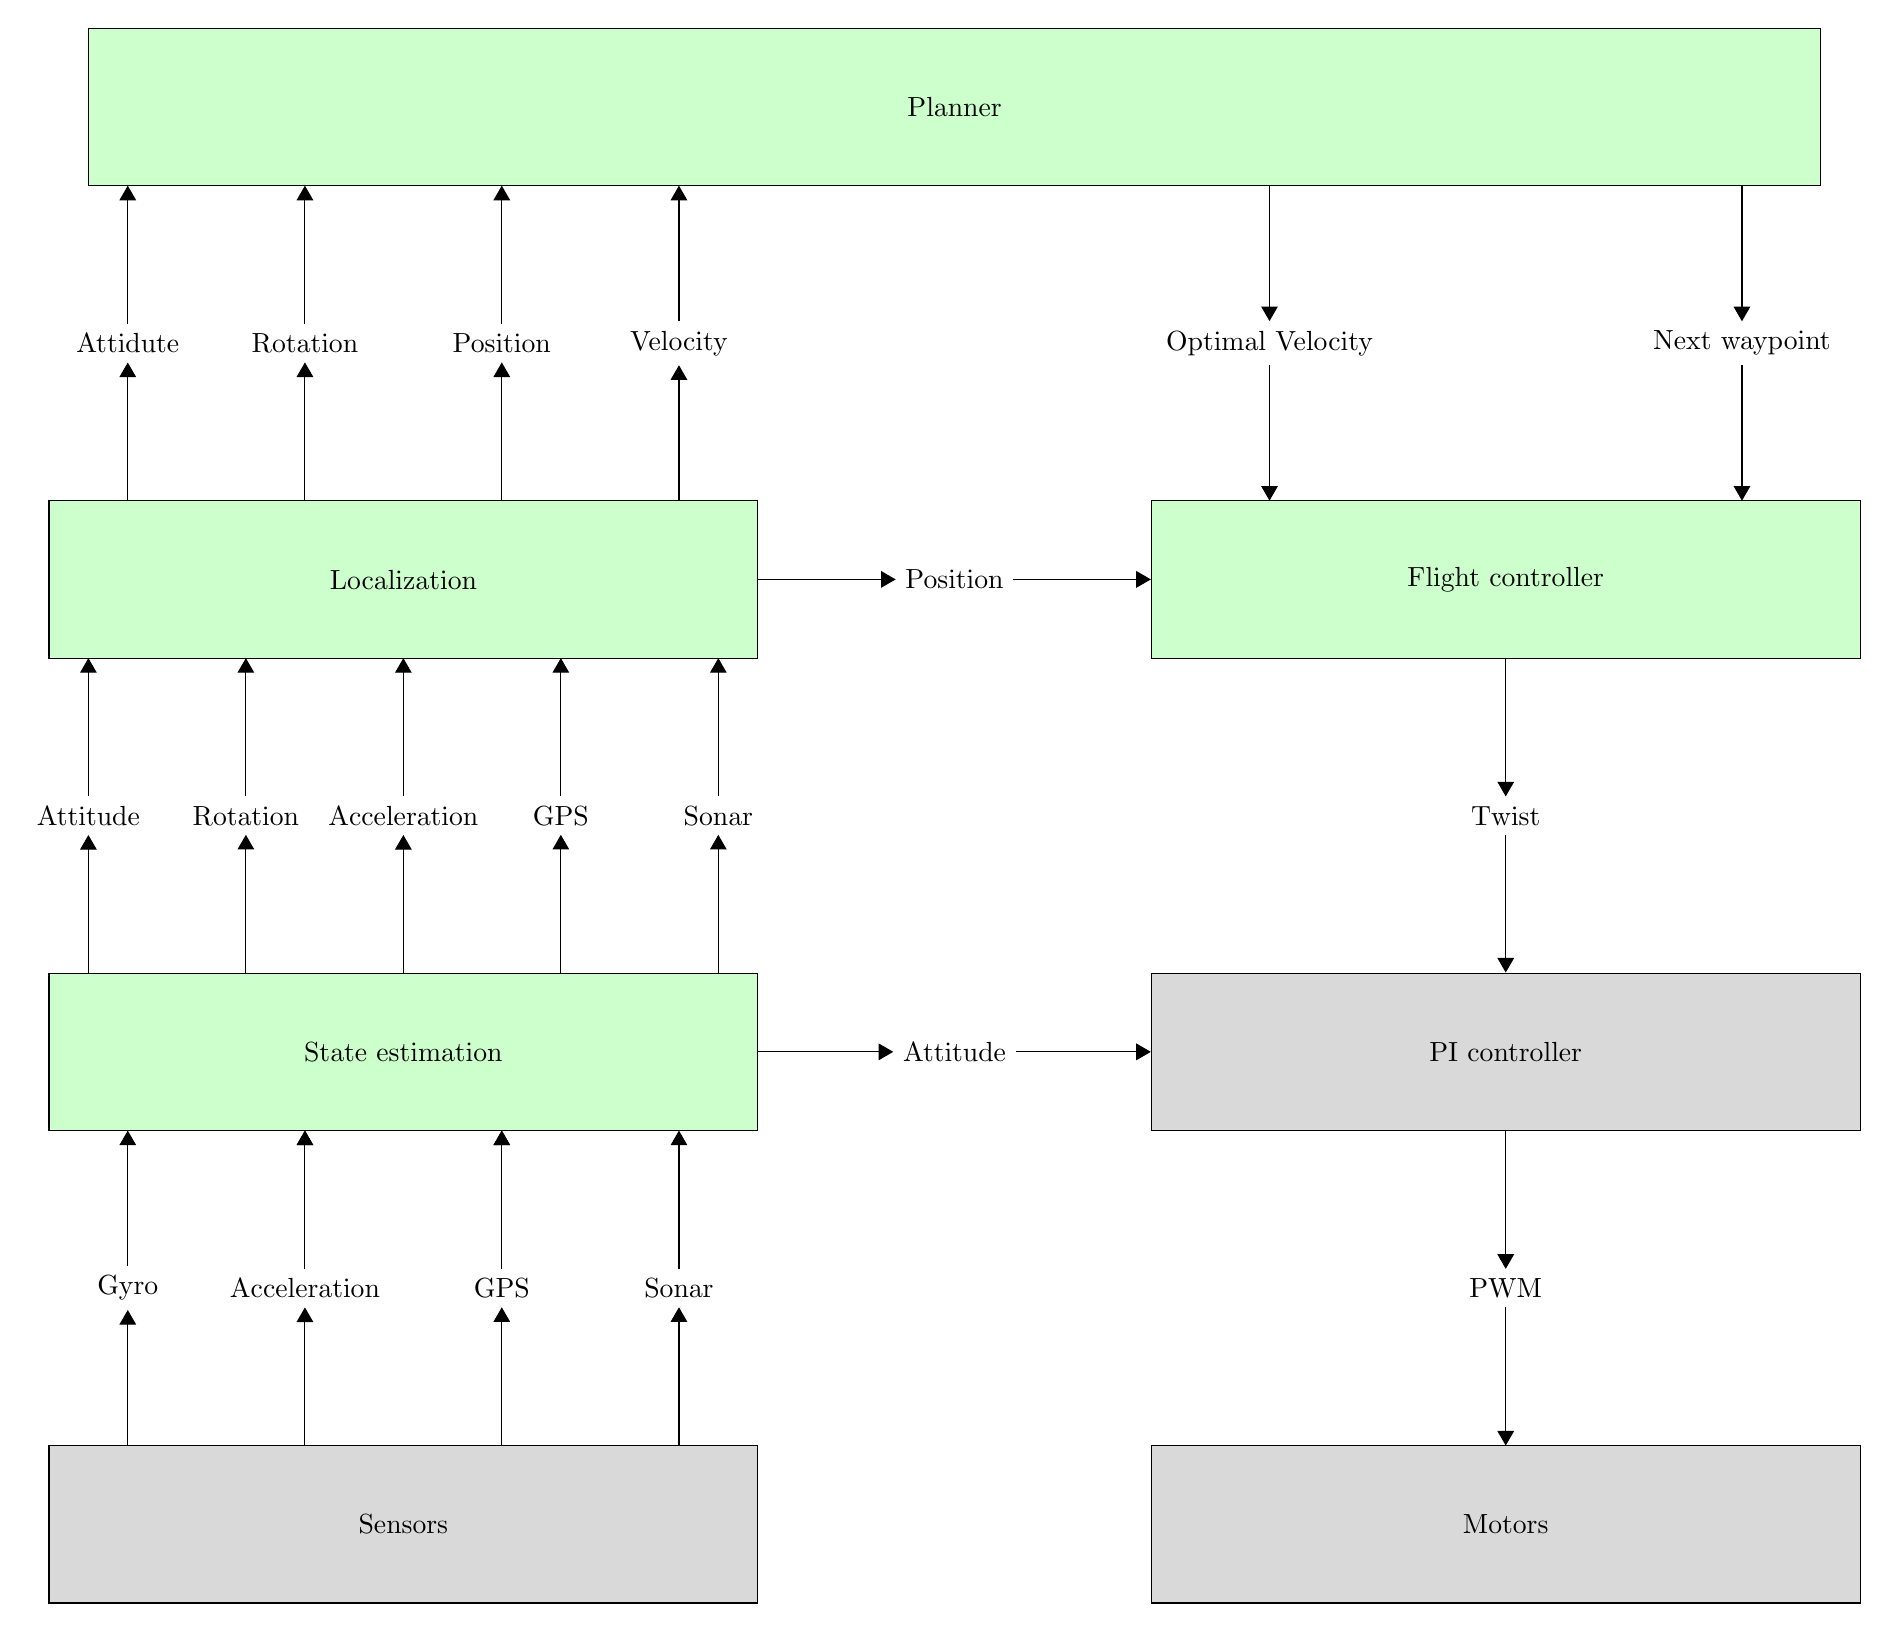
\begin{tikzpicture}
		\node (se1) at (0,0) [draw, fill=green!20,rectangle,minimum width=9cm, minimum height=2cm] {State estimation};
		\node (gyro) at (-3.5, -3) [draw=none] {Gyro};
		\node (acc) at (-1.25, -3) [draw=none] {Acceleration};
		\node (gps) at (1.25, -3) [draw=none] {GPS};
		\node (sonar) at (3.5, -3) [draw=none] {Sonar};
		\node (pose) at (7, 0) [draw=none] {Attitude};
		
		\node (att) at (-4, 3) [draw=none] {Attitude};
		\node (rot) at (-2, 3) [draw=none] {Rotation};
		\node (acc2) at (0, 3) [draw=none] {Acceleration};
		\node (gps2) at (2, 3) [draw=none] {GPS};
		\node (son) at (4, 3) [draw=none] {Sonar};
		
		\draw[-triangle 60] (gyro) to +(0,2);
		\draw[-triangle 60] (acc2) to +(0,2);
		\draw[-triangle 60] (gps2) to +(0,2);
		\draw[-triangle 60] (sonar) to +(0,2);
		\draw[triangle 60-] (pose) to +(-2.5,0);
		
		\draw[triangle 60-] (att) to +(0,-2);
		\draw[triangle 60-] (rot) to +(0,-2);
		\draw[triangle 60-] (acc2) to +(0,-2);
		\draw[triangle 60-] (gps2) to +(0,-2);
		\draw[triangle 60-] (son) to +(0,-2);
	
	\node (se1) at (0,6) [draw, fill=green!20, rectangle,minimum width=9cm, minimum height=2cm] {Localization};
	\node (att2) at (-3.5, 9) [draw=none] {Attidute};
	\node (rot2) at (-1.25, 9) [draw=none] {Rotation};
	\node (pos2) at (1.25, 9) [draw=none] {Position};
	\node (v) at (3.5, 9) [draw=none] {Velocity};
	\node (pos) at (7, 6) [draw=none] {Position};
	

	\draw[-triangle 60] (acc) to +(0,2);
	\draw[-triangle 60] (gps) to +(0,2);
	\draw[-triangle 60] (att) to +(0,2);
	\draw[-triangle 60] (rot) to +(0,2);
	\draw[-triangle 60] (gps) to +(0,2);
	\draw[-triangle 60] (acc) to +(0,2);
	\draw[-triangle 60] (son) to +(0,2);
	\draw[triangle 60-] (pos) to +(-2.5,0);
	
	\draw[triangle 60-] (att2) to +(0,-2);
	\draw[triangle 60-] (rot2) to +(0,-2);
	\draw[triangle 60-] (pos2) to +(0,-2);
	\draw[triangle 60-] (v) to +(0,-2);
	
	\node (pi) at (14,0) [draw, fill=black!15, rectangle,minimum width=9cm, minimum height=2cm] {PI controller};
	\node (fc) at (14,6) [draw, fill=green!20, rectangle,minimum width=9cm, minimum height=2cm] {Flight controller};
	\draw[-triangle 60] (pose) to (pi);
	\draw[-triangle 60] (pos) to (fc);
	\node (twist) at (14,3) [draw=none] {Twist};
	\draw[-triangle 60] (fc) to (twist);
	\draw[-triangle 60] (twist) to (pi);
	
	\node (plan) at (7,12) [draw, fill=green!20, rectangle,minimum width=22cm, minimum height=2cm] {Planner};
	\draw[-triangle 60] (att2) to +(0,2);
	\draw[-triangle 60] (rot2) to +(0,2);
	\draw[-triangle 60] (pos2) to +(0,2);
	\draw[-triangle 60] (v) to +(0,2);
	
	\node (ov) at (11,9) [draw=none] {Optimal Velocity};
	\node (nw) at (17,9) [draw=none] {Next waypoint};
	\draw[triangle 60-] (nw) to +(0,2);
	\draw[triangle 60-] (ov) to +(0,2);
	\draw[-triangle 60] (nw) to +(0,-2);
	\draw[-triangle 60] (ov) to +(0,-2);
	
	\node (sensor) at (0,-6) [draw, fill=black!15,rectangle,minimum width=9cm, minimum height=2cm] {Sensors};
	\draw[triangle 60-] (gyro) to +(0,-2);
	\draw[triangle 60-] (acc) to +(0,-2);
	\draw[triangle 60-] (gps) to +(0,-2);
	\draw[triangle 60-] (sonar) to +(0,-2);
	
	\node (motor) at (14,-6) [draw, fill=black!15,rectangle,minimum width=9cm, minimum height=2cm] {Motors};
	\node (pwm) at (14,-3) [draw=none] {PWM};
	\draw[-triangle 60] (pwm) to +(0,-2);
	\draw[triangle 60-] (pwm) to +(0,2);
	\end{tikzpicture}
	}
	\caption{Interfaces of the control\_system: Gray blocks are already existing, the greens ones have to be implemented}
	\label{fig:state_est}
\end{figure}
\begin{table}
	\centering
	\begin{tabular}{|c|c|c|}\hline
		\textbf{Variable} & \textbf{Components} & \textbf{Range}\\\hline
		Gyro & $\varphi_x, \varphi_y, \varphi_z$ & $\reals \times \reals \times \reals$ \\\hline
		Acceleration & $a_x, a_y, a_z$ &$\reals \times \reals \times \reals$ \\\hline
		GPS & $gps_n, gps_e, gps_d$ & $\reals \times \reals \times \reals$ \\\hline
		Sonar & $s_z$ & $\reals$ \\\hline
		Rotation & $\omega_x, \omega_y, \omega_z$ & $\reals \times \reals \times \reals$ \\\hline
		Attitude & $\theta_x, \theta_y, \theta_z$ & $\reals \times \reals \times \reals$ \\\hline
		Position & $x, y, z$ & $\reals \times \reals \times \reals$ \\\hline
		Velocity & $v_x, v_y, v_z$ & $\reals \times \reals \times \reals$ \\\hline
		Optimal Velocity & $v_{opt}$ & $\reals$ \\\hline
		Next waypoint & $t_x, t_y, t_z$ & $\reals \times \reals \times \reals$ \\\hline
		Twist & $\psi_x, \psi_y, \psi_z$ & $\reals \times \reals \times \reals$ \\\hline
	\end{tabular}
	\caption{Mapping of variables to datatypes}
	\label{tab:datatypes}
\end{table}
The block "state estimation" and "localization" will be implemented as Kalman-filters and have the interfaces as shown in figure (\ref{fig:state_est})
\FloatBarrier
\section*{Task schedule}
	
\end{document}